%%%%%%%%%%%%%%%%%%%%%%%%%%%%%%%%%%%%%%%%%%%%%%%%%%%%%%%%%%%%%%%%%%%%%%%%%%%
% Juan Manuel Perez Rua
%%%%%%%%%%%%%%%%%%%%%%%%%%%%%%%%%%%%%%%%%%%%%%%%%%%%%%%%%%%%%%%%%%%%%%%%%%%

\chapter{Introduction} \label{chap:intro}

Object tracking and optical flow are two of the main components in the
computer vision toolbox, and have been focus of great research efforts, 
leading to significant progress in the last years \cite{c16}\cite{c17}. 
The object tracking problem consist on estimating the 
position of the target in future frames, given an initialization. In the
other hand, the optical flow between a pair of frames consist on finding a motion vector 
for each pixel of interest in the initial image. Even though for several
applications a full motion-field is needed, other applications like
human-computer interaction, object editing in video, non-rigid object interactions in augmented reality, or structure-from-motion,
may only focus on an interest object and, thus, only motion vectors within its 
space may be of interest. 
In such scenarions combining optical flow and object tracking methods in a unified 
framework would become useful and the precision of the object motion description 
could be enhanced. For instance, even with modern optical flow approaches, 
the long term motion problem remains a challenge. However, the problem is more 
bearable for object tracking techniques. In contrast, object trackers are more global 
in motion description, and its information can be completed by optical flow subpixel 
precision. Moreover,  even when object
trackers and optical flow could give good hints for object segmentation in video, 
these elements are not deeply studied in the literature as a unified problem.
We introduce the object flow problem as the computation of dense motion 
flow fields of the set of pixels that belong to an interest object. In other words, 
the object flow by definition induces the segmentation of the target and its motion field.

\section{Problem definition}

We can define more precisely the object flow by starting with an image sequence (See Fig. \ref{diagram} for a simple diagram) and an initial 
position of the interest object in the first frame of this sequence, and letting $\mathcal{R}$ 
be the region corresponding to the support of the object in 2D, such that 
$\mathcal{R} \subset \Omega$. If $\Omega$ is the set of all the possible grid positions, 
the object flow problem consist in finding the displacement vectors $d_{0,t}(x)$ from the image $I_{0}$ to $I_{t}$, $\forall x \in \mathcal{R}$.

   \begin{figure}[bhp]
      \centering
      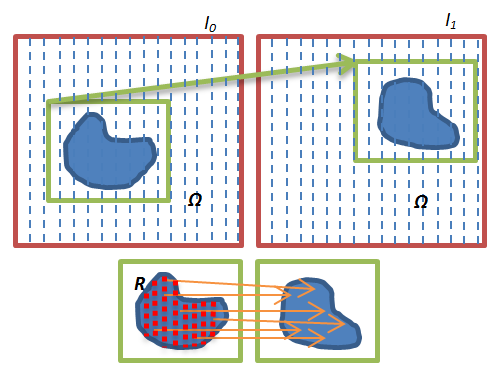
\includegraphics[width=0.66\textwidth]{../images/diagram.png}
      \caption{ Object flow definition diagram. }
      \label{diagram}
   \end{figure}

A straightforward solution to this problem would be to compute the optical flow motion field, and apply 
a segmentation mask to recover the desired motion vectors. Nevertheless, this approach carries several 
problems. For example, a globally computed optical flow method can affect small objects motion, because of 
the common use of heavy regularization priors. Moreover, even if the segmentation mask is extracted from a 
tracker window by a graph-cut based segmentation method, is likely that this mask is not going to be well suited for the 
interest object and some extra user interaction would be needed to refine this process. We propose an approach 
to reduce these problems.

\section{Objectives}

The main goal of this work is to define a dense motion descriptor for objects in video sequences. 
In order to achieve this goal, some specific objectives are defined:

\begin{itemize}

  \item To show experimentally that the idea of mixing tracking techniques with optical flow methods enhance the precision of per-object motion description.
  \item To define an automatic segmentation approach for target objects in video sequences.
  \item To establish a flow estimation method that uses the segmentation mask provided and the region of interest given by the tracker.
  \item To show experimentally that the proposed object flow method is indeed more precise than regular optical flow techniques.

\end{itemize}

\section{Document organization}

The section \ref{chap:background} starts by introducing the reader in the important topics and concepts that support the rest of this work: 
object tracking, optical flow and object segmentation. After this, in the section \ref{chap:core}, the object flow pipeline is explained in deep, 
together with the proposed algorithms. Finally, a list of results and implementation details are discussed in \ref{chap:results}.


